\documentclass{beamer}
\usepackage[utf8]{inputenc}

\usetheme{Madrid}
\usecolortheme{default}
\usepackage{amsmath,amssymb,amsfonts,amsthm}
\usepackage{txfonts}
\usepackage{tkz-euclide}
\usepackage{listings}
\usepackage{adjustbox}
\usepackage{array}
\usepackage{tabularx}
\usepackage{gvv}
\usepackage{lmodern}
\usepackage{circuitikz}
\usepackage{tikz}
\usepackage{graphicx}

\setbeamertemplate{page number in head/foot}[totalframenumber]

\usepackage{tcolorbox}
\tcbuselibrary{minted,breakable,xparse,skins}



\definecolor{bg}{gray}{0.95}
\DeclareTCBListing{mintedbox}{O{}m!O{}}{%
  breakable=true,
  listing engine=minted,
  listing only,
  minted language=#2,
  minted style=default,
  minted options={%
    linenos,
    gobble=0,
    breaklines=true,
    breakafter=,,
    fontsize=\small,
    numbersep=8pt,
    #1},
  boxsep=0pt,
  left skip=0pt,
  right skip=0pt,
  left=25pt,
  right=0pt,
  top=3pt,
  bottom=3pt,
  arc=5pt,
  leftrule=0pt,
  rightrule=0pt,
  bottomrule=2pt,
  toprule=2pt,
  colback=bg,
  colframe=orange!70,
  enhanced,
  overlay={%
    \begin{tcbclipinterior}
    \fill[orange!20!white] (frame.south west) rectangle ([xshift=20pt]frame.north west);
    \end{tcbclipinterior}},
  #3,
}
\lstset{
    language=C,
    basicstyle=\ttfamily\small,
    keywordstyle=\color{blue},
    stringstyle=\color{orange},
    commentstyle=\color{green!60!black},
    numbers=left,
    numberstyle=\tiny\color{gray},
    breaklines=true,
    showstringspaces=false,
}
%------------------------------------------------------------

\title
{5.2.70}
\date{September 12,2025}
\author 
{AI25BTECH11003 - Bhavesh Gaikwad}



\begin{document}


\frame{\titlepage}
\begin{frame}{Question}
For which values of p does the pair of equations given below have a unique solution.
\begin{center}
4x + py + 8 = 0 \\
2x + 2y + 2 = 0 
\end{center}
\end{frame}


\begin{frame}[fragile]
    \frametitle{Theoretical Solution}
    Given:
\begin{align}
4x + py + 8 &= 0 \\
2x + 2y + 2 &= 0
\end{align}

Standard Form: $ \vec{A}\vec{x} = \vec{b} $ where:\\\\
Coefficient Matrix: $ \vec{A} = \myvec{4 & p \\ 2 & 2} $\\\\
Constant Vector: $ \vec{b} = \myvec{-8 \\ -2} $\\\\
Augmented Matrix: $ [\vec{A}|\vec{b}] = \myvec{4 & p & -8 \\ 2 & 2 & -2} $
\end{frame}



\begin{frame}[fragile]
    \frametitle{Theoretical Solution}
For Unique Solution:\\
Unique Solution: $ \rank(\vec{A}) = \rank([\vec{A}|\vec{b}]) = n $ (number of variables)\\
For our system: $ n = 2 $ variables\\\\

Finding $\rank(\vec{A})$ - Rank of Coefficient Matrix\\

Initial Matrix $ \vec{A} $:
\begin{equation}
\vec{A} = \myvec{4 & p \\ 2 & 2}
\end{equation}

Row Operations on $\vec{A}$:
\begin{align}
R_2 &\to R_2 - \frac{1}{2}R_1
\end{align}

Row Echelon Form of $ \vec{A} $:
\begin{equation}
\myvec{4 & p \\ 0 & 2 - \tfrac{p}{2}}
\end{equation}
\end{frame}



\begin{frame}[fragile]
    \frametitle{Theoretical Solution}
Rank Analysis:\\
    Case 1: If $ 2 - \dfrac{p}{2} \neq 0 $ (i.e., $ p \neq 4 $)\\
        Both rows are non-zero and linearly independent \\
        $ \Rightarrow \rank(\vec{A}) = 2 $\\\\
Case 2: If $ 2 - \dfrac{p}{2} = 0 $ (i.e., $ p = 4 $)\\
        Second row is zero, only first row is non-zero \\
        $ \Rightarrow \rank(\vec{A}) = 1 $
\bigskip

Finding $\rank([\vec{A}|\vec{b}])$ - Rank of Augmented Matrix

Initial Augmented Matrix:
\begin{equation}
\myvec{4 & p & -8 \\ 2 & 2 & -2}
\end{equation}
\end{frame}

\begin{frame}[fragile]
    \frametitle{Theoretical Solution}
Row Operation on $[\vec{A}|\vec{b}]$:\\ 
\begin{align}
R_2 \to R_2 - \frac{1}{2}R_1
\end{align}

Row Echelon Form of Augmented Matrix:
\begin{equation}
\myvec{4 & p & -8 \\ 0 & 2-\frac{p}{2} & 2}
\end{equation}

Rank Analysis:\\
Case 1: If $ p \neq 4 $:\\
$\Rightarrow \rank([\vec{A}|\vec{b}]) = 2$\\

Case 2: If $ p = 4 $:\\
$ \Rightarrow \rank([\vec{A}|\vec{b}]) = 2 $\\\\
\end{frame}

\begin{frame}[fragile]
    \frametitle{Theoretical Solution}
Comparing Ranks and Providing Solution Type
\begin{center}
\begin{tabular}[12pt]{ |c| c|}
    \hline
    \textbf{Variable} & \textbf{value}\\ 
    \hline
    \textbf{$A$} & $\myvec{1\\-3}$\\
    \hline
 \textbf{$B$} & $\myvec{4\\p}$\\
    \hline
 \textbf{$C$} & $\myvec{-9\\7}$\\
    \hline
    \end{tabular}
\end{center}

\begin{align}
\boxed{\therefore \, \text{For p} \, \epsilon \, \mathbb{R}-\{4\}, \, \text{the pair of equations has an Unique Solution.}}
\end{align}
\end{frame}


\begin{frame}{Graph of Pair of Equations (When p=4)}
   \centering
    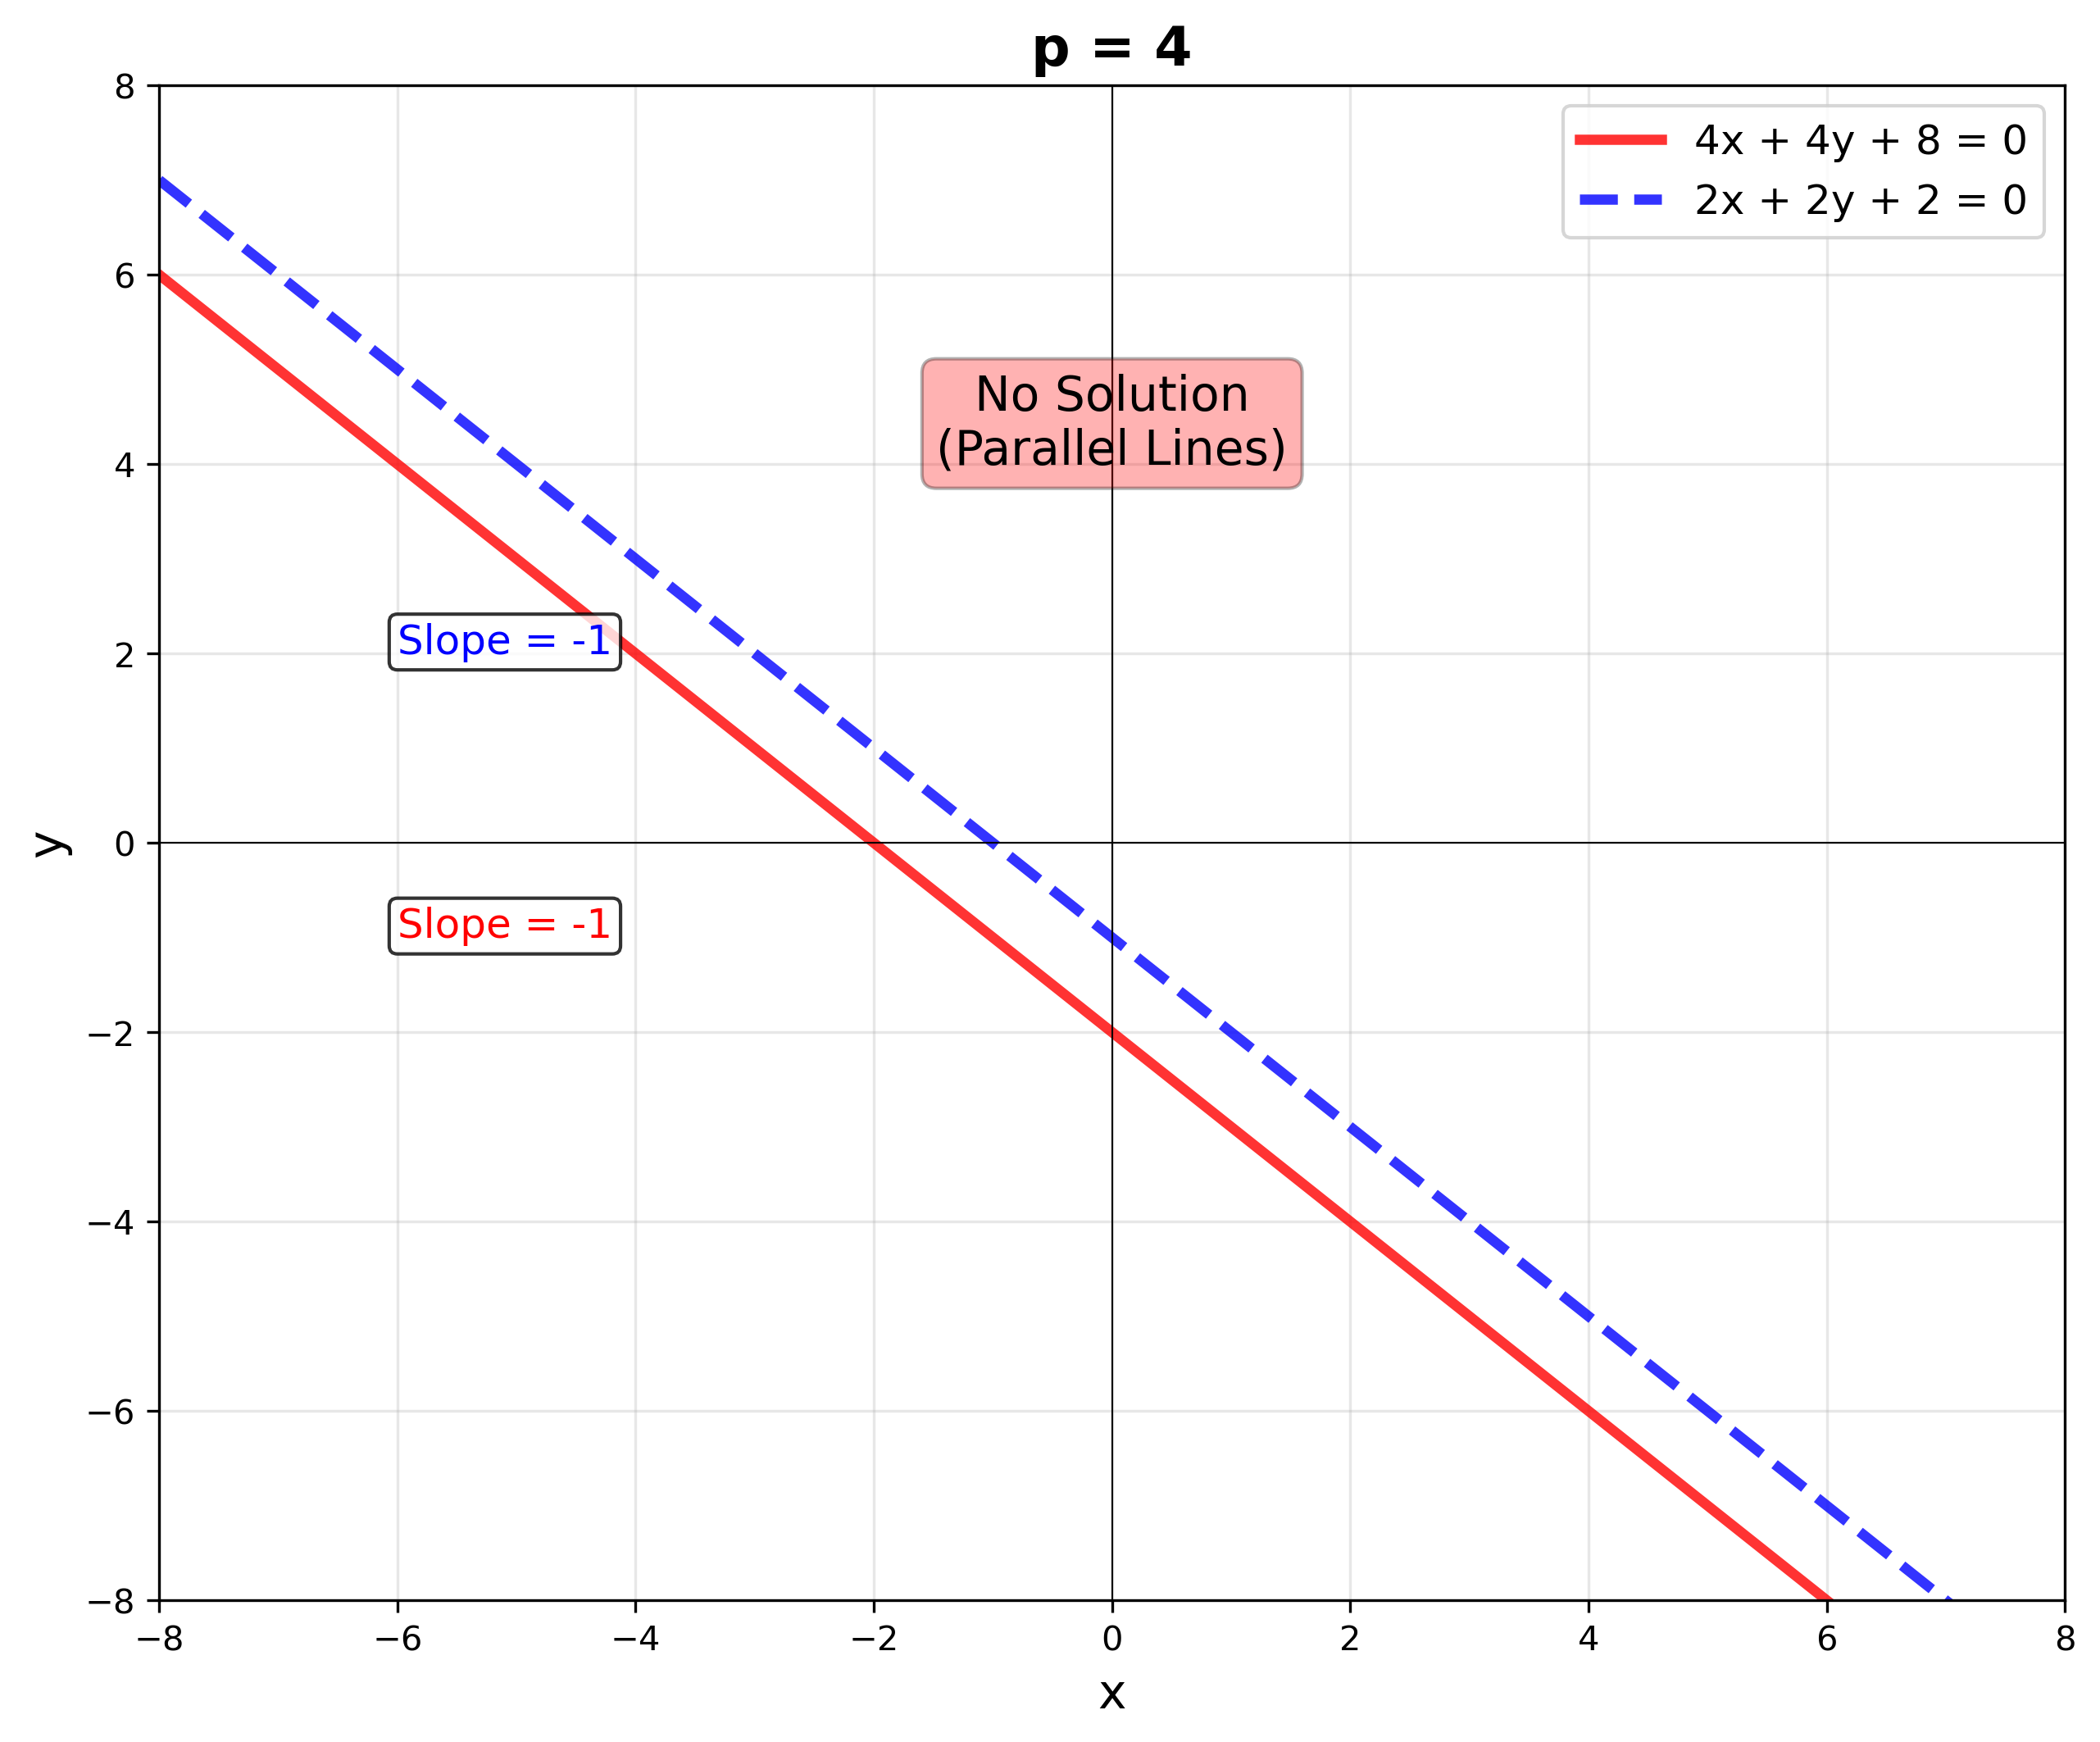
\includegraphics[width=\columnwidth, height=0.8\textheight, keepaspectratio]{figs/fig1.png}
    \label{fig:Beamer/figs/fig1.png}
\end{frame}

\begin{frame}{Graph of Pair of Equations (When p$\neq$4)}
   \centering
    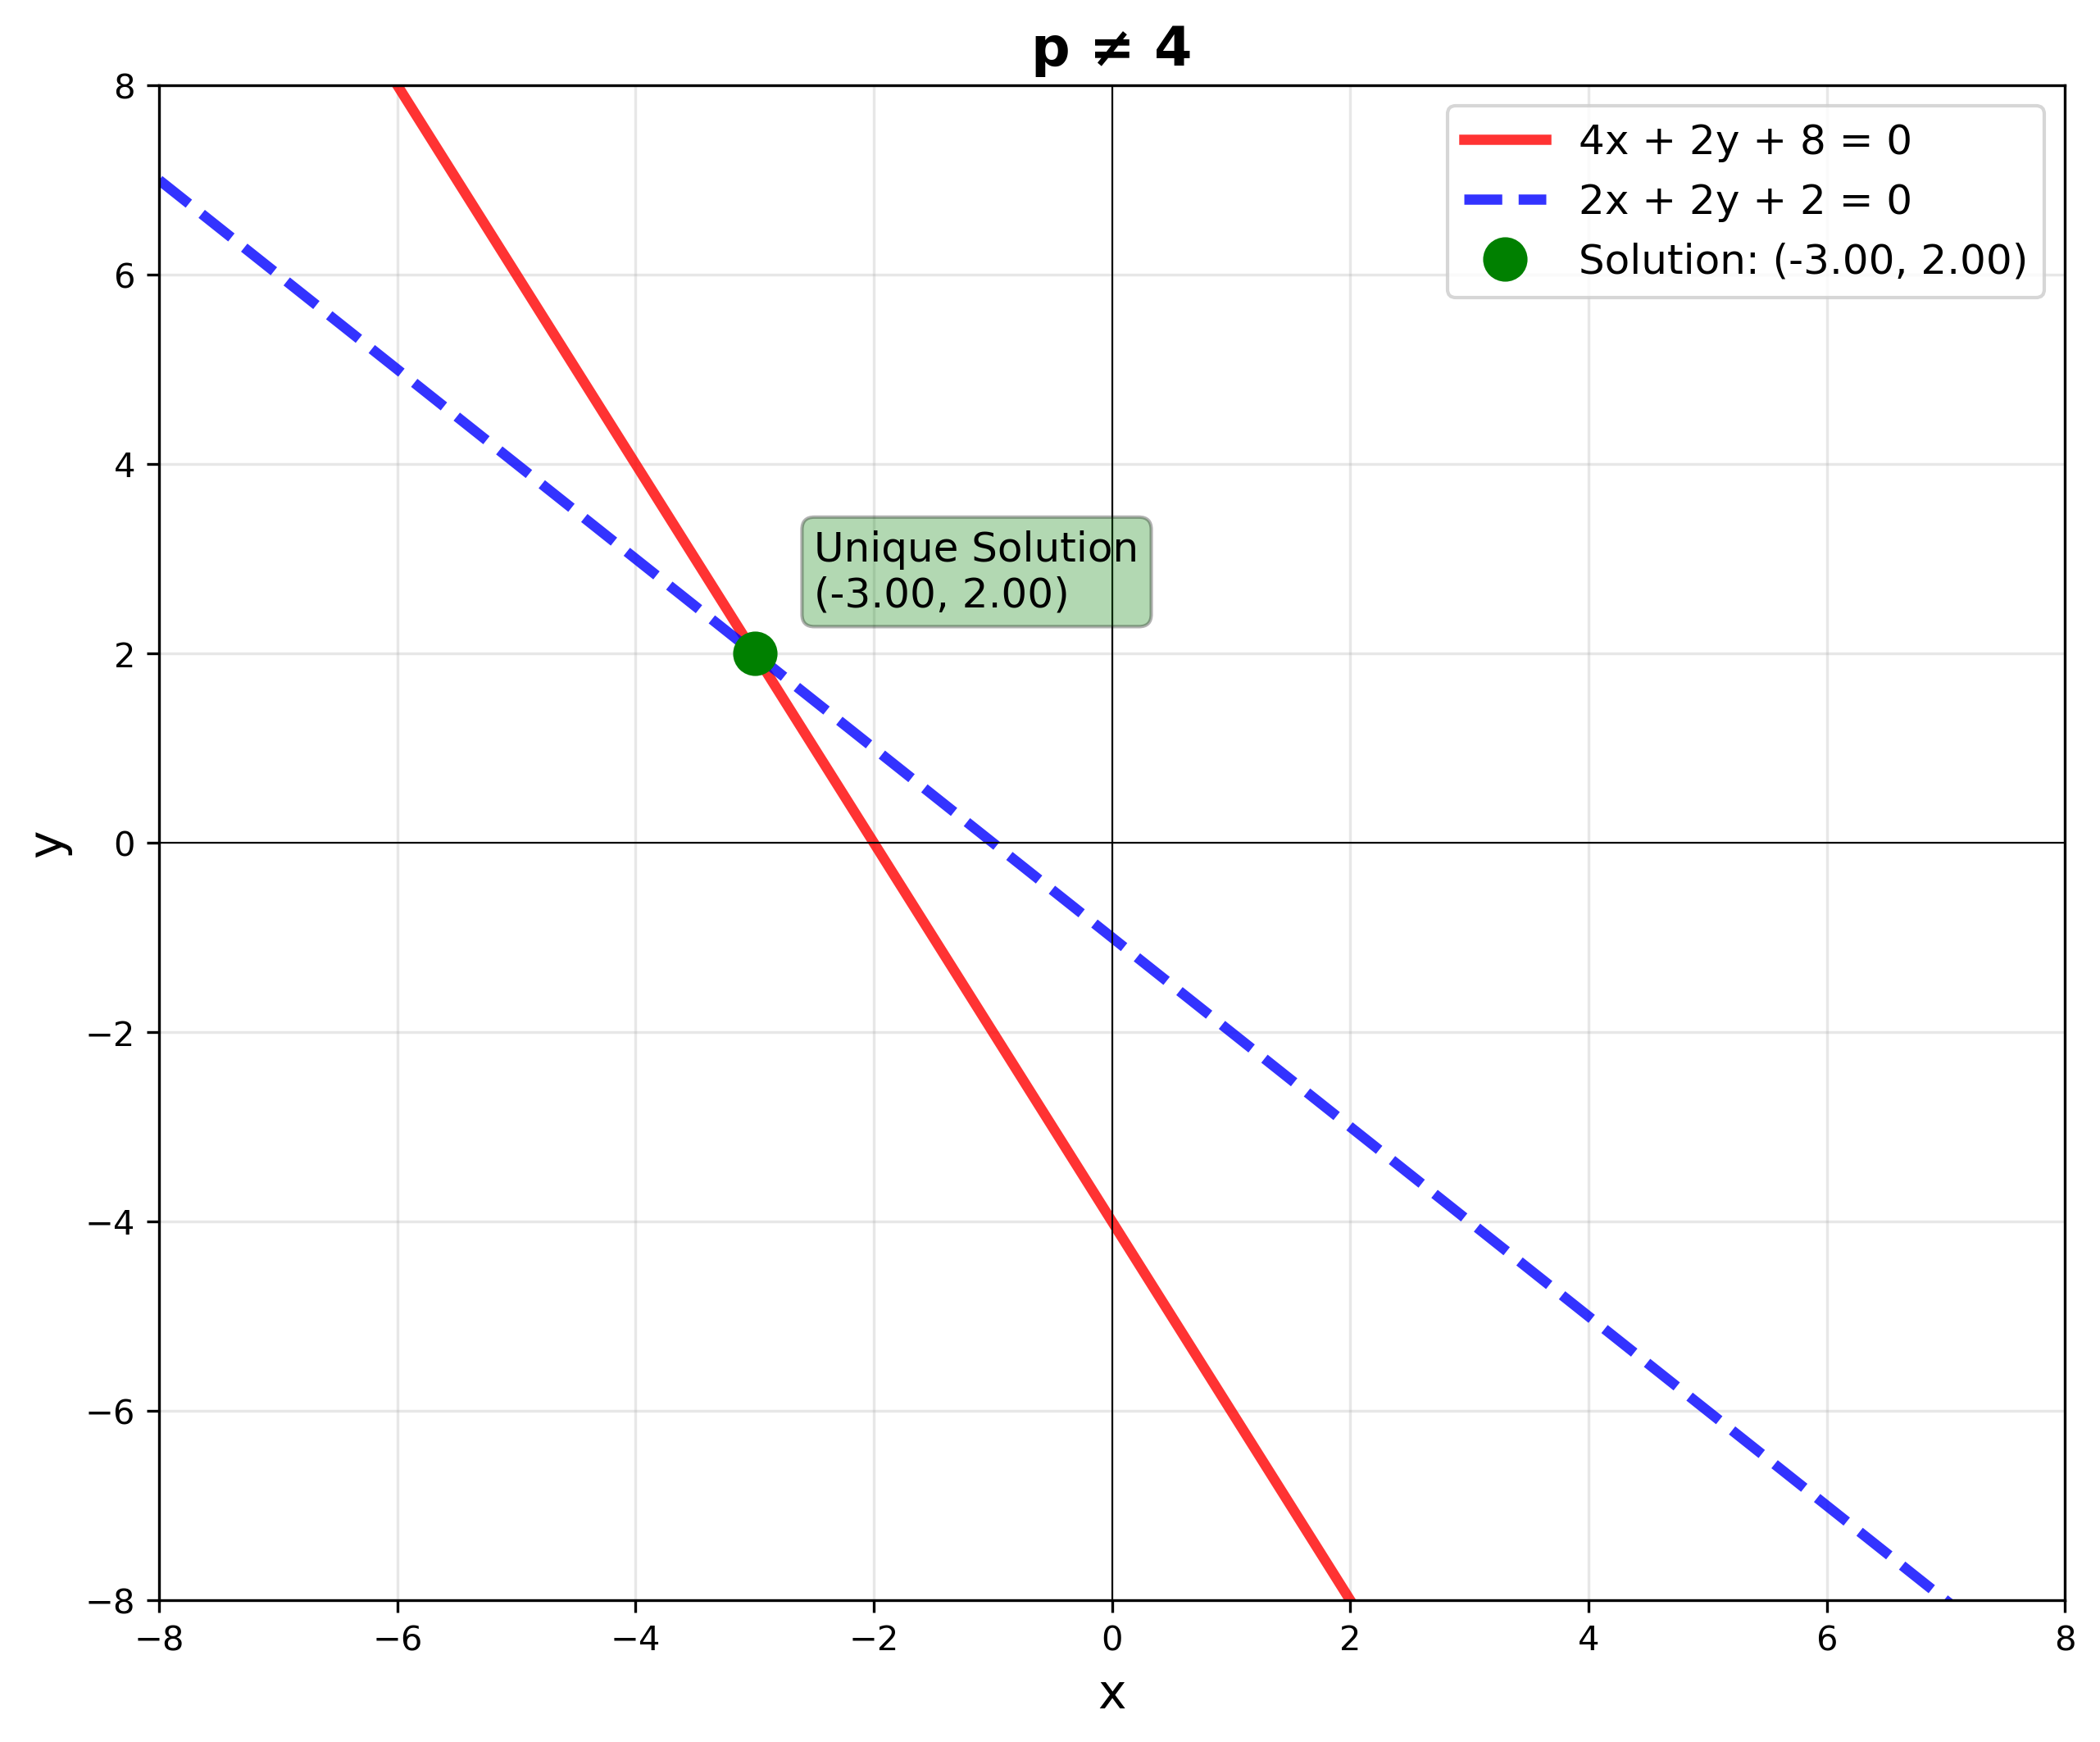
\includegraphics[width=\columnwidth, height=0.8\textheight, keepaspectratio]{figs/fig2.png}
    \label{fig:Beamer/figs/fig2.png}
\end{frame}
\end{document}